\documentclass[11pt,a4paper]{article}
\usepackage{fontspec}
\setmainfont{Source Serif 4}[Path=/home/claude/ref/fonts/, UprightFont=SourceSerif4-Regular.ttf, BoldFont=SourceSerif4-Semibold.ttf, ItalicFont=SourceSerif4-It.ttf]
\setmonofont{IBM Plex Mono}[Path=/home/claude/ref/fonts/, UprightFont=IBMPlexMono-Regular.ttf, BoldFont=IBMPlexMono-Medium.ttf, Scale=0.88]
\usepackage[a4paper,margin=2.4cm]{geometry}
\usepackage{amsmath}
\usepackage{graphicx,booktabs,float,caption,array,xcolor,longtable}
\usepackage{xurl}
\usepackage[hidelinks]{hyperref}
\usepackage[round]{natbib}
\usepackage{setspace}
\setstretch{1.08}
\renewcommand{\topfraction}{0.9}
\renewcommand{\bottomfraction}{0.8}
\renewcommand{\textfraction}{0.1}
\renewcommand{\floatpagefraction}{0.75}
\setlength{\parindent}{0pt}
\setlength{\parskip}{0.55em}
\captionsetup{font=small,labelfont=bf}
\setlength{\bibsep}{3pt}
\urlstyle{same}
\hypersetup{pdftitle={Who Owns Your Street?},pdfauthor={Dr Tristan Hotham}}

\begin{document}
\begin{center}
{\Large\bfseries Who Owns Your Street? The Small-Area Geography of Property in England and Wales Held by Overseas Companies\par}
\vspace{1.2em}
{\large Dr Tristan Hotham\par}
\vspace{0.3em}
{\small Independent researcher\\
ORCID: 0000-0003-4931-9349\\
DOI: https://doi.org/10.5281/zenodo.24115198\par}
\vspace{0.8em}
2026
\end{center}

\begin{quote}
\small
\begin{center}\textbf{Abstract}\end{center}
Debates about offshore ownership of British property have focused on prime central London and on a few headline totals. This paper maps the whole register. Using HM Land Registry's full file of property titles in England and Wales whose legal owner is a company incorporated overseas (November 2026; 90,949 titles), I place 66,913 titles in small areas (LSOAs) and relate them to the Council Tax housing stock. Following an analysis plan written before any counts were computed, I test three expectations. First, the titles are far more concentrated than homes: the Gini coefficient across 35,672 small areas is 0.87, against 0.14 for dwellings, and half of the titles placed in small areas sit in 2.1\% of small areas. Second, 75.7\% of titles are held by companies incorporated in the UK's Crown Dependencies and Overseas Territories, led by Jersey, the British Virgin Islands, Guernsey and the Isle of Man. Third, comparing small areas within the same district, titles are more common where more homes are in the top Council Tax bands (rate ratio 1.29 per 10 percentage points), where more homes are flats (1.30) and where more were built since 2009 (1.10). These associations hold in a negative binomial model, without London, by tenure and for flats alone, and a within-district placebo centres on 1. The pattern is descriptive: the register records legal owners, not beneficial owners, uses or motives, and covers only companies incorporated abroad.

\textbf{Keywords:} offshore ownership; real estate; tax havens; financial secrecy; housing; small-area geography; England and Wales
\end{quote}

\section{Introduction}\label{sec:intro}
The ownership of British property by companies registered in other jurisdictions has become a political subject. Campaign reports have described London property as a destination for illicit wealth \citep{tiuk2015,tiuk2017}; urban scholars have described the city's prime residential districts as a ``safe deposit box'' for a transnational wealth elite \citep{fernandez2016} and its richest neighbourhoods as ``alpha territories'' reshaped by the super-rich \citep{webber2016,burrows2017,atkinson2020}; and Parliament responded in 2022 by requiring overseas entities that own land in the UK to disclose their beneficial owners \citep{ecta2022}. Economists, meanwhile, have used the register of overseas-company titles that HM Land Registry publishes to estimate the effect of foreign investment on house prices \citep{sa2025}, the response of offshore buyers to international tax transparency \citep{bomare2022}, and the effect of the 2022 beneficial ownership rules on purchases by companies in tax havens \citep{collin2025}.

Much of this work studies either a single city, typically London, or a flow of purchases through time. Less is known about the plain geography of the stock: where, across the whole of England and Wales and at a fine scale, the titles held by overseas companies actually are; how concentrated they are; which jurisdictions the companies come from; and what kind of neighbourhood they tend to be in. This paper provides that description. It uses the full HM Land Registry file for November 2026, places each title in its Lower layer Super Output Area (LSOA, a small area of about 1,500 residents) from its postcode, and relates the counts to the Valuation Office Agency's count of dwellings and its description of the housing stock in each area.

The analysis was pre-specified in a written plan before any counts were made. It has three parts. The first measures concentration: how unevenly titles are spread across districts and small areas compared with homes. The second describes jurisdictions: what share of titles are held by companies incorporated in the Crown Dependencies and British Overseas Territories, a group with a particular constitutional relationship to the UK and a central place in the literature on offshore finance \citep{palan2010,shaxson2011,haberly2015a}. The third asks, within districts, what kind of small area has more overseas-company titles per home: areas with more homes in the top Council Tax bands, more flats, or more recently built homes.

The main results are simple to state. Overseas-company titles are extremely concentrated. Westminster and Kensington and Chelsea hold 16.0\% of all titles with 0.8\% of homes, and London as a whole 42.8\% of titles with 14.1\% of homes. Yet titles are also widespread: 39\% of small areas contain at least one. 75.7\% of titles are held by companies from the Crown Dependencies and Overseas Territories, and the share is higher outside London than inside it. Within districts, titles are more common in areas with more expensive, flatted and newer housing, a pattern that is stable across every planned check.

The paper makes three contributions. It gives the first complete small-area map, for all of England and Wales, of the overseas-company register expressed as a rate per home, and publishes the aggregate counts so that others can use them without handling the title-level file. It brings the jurisdiction mix of the register into contact with the literature on secrecy jurisdictions and offshore networks \citep{cobham2015,garcia2017}, showing how far the UK's own offshore satellites dominate the register. And it tests, with a transparent within-district design, which kinds of neighbourhood hold these titles outside the familiar prime districts. The design is descriptive. It does not identify why companies hold property where they do, nor who stands behind them.

Section~\ref{sec:lit} reviews the literature on offshore ownership, foreign investment in housing and the geography of elite property. Section~\ref{sec:data} describes the data and Section~\ref{sec:design} the design. Section~\ref{sec:results} reports the results and Section~\ref{sec:robust} the robustness checks. Section~\ref{sec:disc} discusses what the pattern means and what it cannot show, and Section~\ref{sec:conc} concludes.

\section{Background and literature}\label{sec:lit}
\subsection{Offshore wealth and secrecy jurisdictions}
A large literature documents the scale and structure of wealth held offshore. \citet{zucman2013} estimated from anomalies in international investment positions that around 8\% of global household financial wealth is held in tax havens, and \citet{alstadsaeter2018} showed that ownership of this wealth is highly concentrated at the top of national wealth distributions. Policy responses aimed at bank secrecy have had mixed effects: \citet{johannesen2014} found that the G20's bilateral information exchange treaties shifted deposits towards non-compliant havens rather than repatriating them. Property is a natural place for such wealth to go, because it was outside the scope of the automatic exchange of financial account information. \citet{bomare2022} used the HM Land Registry overseas-company data and leaked ownership records to show that purchases of UK property by companies from the havens most exposed to the Common Reporting Standard rose after it was introduced.

Which jurisdictions count as offshore is itself a research question. The Tax Justice Network's Financial Secrecy Index scores jurisdictions on the secrecy of their legal and financial systems and weights them by their share of cross-border financial services \citep{cobham2015,tjn2018}. Network studies of corporate ownership distinguish ``conduit'' jurisdictions, through which ownership chains pass, from ``sink'' jurisdictions, where value comes to rest \citep{garcia2017}, and show that offshore investment forms regional blocks with strong imperial legacies, with the British Crown Dependencies and Overseas Territories at the centre of one of them \citep{haberly2015a,haberly2015b}. Historical and journalistic accounts describe the same network as a ``second British empire'' of finance centred on the City of London \citep{palan2010,shaxson2011}. The professional work that makes these structures possible, by wealth managers, lawyers and trust companies, has been described by \citet{harrington2016}.

\subsection{Foreign and offshore investment in housing}
A second literature asks what foreign investment does to housing markets. \citet{badarinza2018} used political and economic shocks abroad as a source of variation in foreign demand for London housing, and found that such shocks raised prices in the areas of London where buyers from the affected countries had historically bought. \citet{sa2025}, using the same HM Land Registry register as this paper aggregated to local authorities, found that foreign investment raised house prices across the whole price distribution, reduced affordability and reduced the number of empty homes, with no measurable effect on construction. In the United States, \citet{gorback2020} exploited foreign buyer taxes introduced in other countries and found that foreign capital raised local house prices and modestly increased supply. These studies treat foreign investment as a cause and house prices as an effect. This paper asks a prior, descriptive question: in what kind of neighbourhood are overseas-company titles located?

Sociologists and geographers have written about the people behind these flows and their effects on cities. \citet{fernandez2016} described London and New York as safe deposit boxes for a transnational wealth elite, organised through offshore financial centres and valued for liquidity and legal security. \citet{rogers2017} introduced a collection on the globalisation of real estate, and \citet{ley2017} traced how Chinese capital and immigration reshaped Vancouver's housing market. \citet{wetzstein2017} placed such investment within a global urban crisis of housing affordability, and \citet{aalbers2016} within the financialisation of housing more generally.

\subsection{Elite property in London}
London is the most studied case. \citet{webber2016} described life in an ``alpha territory'', and \citet{burrows2017} mapped such territories across the city using geodemographic data. \citet{atkinson2017} and \citet{atkinson2020} argued that the city's policy of welcoming capital and the very rich has produced a ``minimum city'' in which concentrated wealth pulls away from shared provision and public space. \citet{knowles2022} walked the streets of plutocratic London to describe how these flows appear on the ground. Campaign groups have tried to measure the part that anonymous and possibly corrupt money plays. \citet{tiuk2015} argued that UK property was attractive to corrupt capital and that companies in secrecy jurisdictions made buyers hard to trace, and \citet{tiuk2017} examined new landmark developments in London and found a large share of homes sold to investors from high corruption risk countries or through anonymous companies.

The overseas-company register itself has been extended and classified by \citet{bourne2022}, who combined it with other sources and machine learning to enlarge it to about 138,000 properties classified by use, most of them residential and many in London, and found that offshore-owned residential property in London is more expensive and more spatially concentrated than Airbnb, low-use and conventional homes. \citet{collin2025} used the register to show that, after the Register of Overseas Entities was introduced in 2022, new purchases by companies in tax havens fell relative to purchases by companies elsewhere.

\subsection{Contribution and expectations}
The existing work has mostly measured flows through time, focused on London, or aggregated to local authorities. What is missing is a description of the stock at a fine spatial scale for the whole of England and Wales, expressed relative to the number of homes, and an account of what kind of small area holds the titles once the strong differences between districts are set aside. The literature suggests three expectations, which I wrote down before computing any counts. First (H1), the titles should be far more concentrated than homes, with the highest district rates in Westminster and Kensington and Chelsea, the core of London's prime market \citep{fernandez2016,burrows2017}. Second (H2), more than half of titles should be held by companies from the UK-linked offshore jurisdictions \citep{haberly2015a,bomare2022}. Third (H3), within districts, titles should be more common in small areas with more homes in the highest Council Tax bands (the prime-market expectation), more flats (the investment-unit expectation, since flats are the typical product of investor-oriented development; \citealp{tiuk2017}) and more homes built since 2009 (the new-build expectation, since new developments are often marketed to investors, as in the developments studied by \citealp{tiuk2017}).

\section{Data}\label{sec:data}
\subsection{Overseas-company titles}
HM Land Registry publishes a list of registered freehold and leasehold titles in England and Wales whose registered proprietor is a company incorporated outside the UK \citep{hmlr2026}. Titles registered to private individuals, UK companies with an overseas address and charities are excluded by the publisher. I use the full file dated November 2026, which has 90,950 rows and 39 columns: the title number, tenure, property address, district, county, region, postcode, a multiple address indicator, the price paid where recorded, up to four proprietors with their company registration number, proprietorship category, country of incorporation and address, and the date the current proprietor was added. One malformed row with no tenure and no proprietor is dropped, leaving 90,949 titles.

The file is licensed for non-commercial use, and the licence forbids publishing the information as a standalone product. I therefore publish only aggregates: counts by small area, district, region, jurisdiction, tenure and year, price summaries for groups of at least ten titles, and the number of titles held by the ten largest corporate proprietors. No title number, address or postcode appears in any output. Information produced by HM Land Registry \textcopyright{} Crown copyright 2026.

A title is a unit of legal registration, not a dwelling. It can be a flat, a house, a shop, an office building, a parcel of land, or (for 757 titles flagged as having multiple addresses) several properties at once. Results are therefore stated in titles throughout. As a rough guide to how many are homes, 22.4\% of titles have an address containing ``flat'', ``apartment'', ``maisonette'', ``studio'' or ``penthouse'' (37\% in London, 11\% elsewhere); this undercounts houses and is used only as a robustness check. 45.2\% of titles are leasehold.

\subsection{Places and jurisdictions}
Each title's postcode was matched to the postcodes.io lookup of the ONS Postcode Directory, which gives its 2021 LSOA and local authority district. 66,913 titles (73.6\%) have a postcode that matches; 21,669 have no postcode, often land or multiple properties, and 2,367 have a postcode that is no longer current or is mistyped. These 24,036 titles are assigned to a district from the file's own district field (using the district in which titles with the same district name and a valid postcode most often fall) and enter district totals but not the small-area analysis. Every title has a district.

The country of incorporation is recorded as free text. The first proprietor's value has 207 distinct spellings. I map American states to the United States, Canadian provinces to Canada, the individual emirates and free zones to the United Arab Emirates and Alderney to Guernsey, and correct misspellings, leaving 131 named jurisdictions and a handful of vague labels (``Channel Islands'', ``The Virgin Islands'', ``The West Indies''). The UK-linked offshore jurisdictions are defined in advance on constitutional grounds: the Crown Dependencies (Jersey, the Bailiwick of Guernsey and the Isle of Man, plus unspecified ``Channel Islands'') and the British Overseas Territories that appear in the file (the British Virgin Islands, the Cayman Islands, Bermuda, Gibraltar, Anguilla, the Turks and Caicos Islands and Montserrat). As a secondary classification I use the Financial Secrecy Index secrecy scores \citep{tjn2018}; the most recent edition that is available in a reusable form is 2018, and it covers jurisdictions holding 97.9\% of titles.

\subsection{Homes and neighbourhoods}
The denominator is the number of dwellings on the Council Tax valuation list in each LSOA at 31 March 2025, from the Valuation Office Agency's stock of properties statistics \citep{voa2025}, which total 27,248,070 across England and Wales. The same tables describe each area's housing: the number of dwellings in each Council Tax band and build period (table CTSOP4.1) and the number of flats and maisonettes (table CTSOP3.1). From these I compute three shares: the share of dwellings in the top three bands (F to H in England, G to I in Wales, where the band scale has nine bands); the share of flats and maisonettes; and the share of dwellings of known age built in 2009 or later. Council Tax bands reflect values in 1991 in England and 2003 in Wales, so they describe the relative value of the stock rather than current prices, but they are available for every small area. Counts are rounded to the nearest ten by the VOA and counts below five are suppressed; I treat suppressed cells as zero and, as a check, as 2.5.

\subsection{Boundaries}
LSOA 2021 boundaries come from the ONS generalised clipped files \citep{ons2021lsoa}, through the GitHub copy in the drkane/geo-lookups repository, and district boundaries from the ONS December 2023 file. Table~\ref{tab:data} summarises the data flow.

\begin{table}[tbp]\centering\small\caption{Data flow.}\label{tab:data}\begin{tabular}{lr}\toprule Item & Number\\\midrule
Rows in the HM Land Registry file (November 2026) & 90,950\\
\quad malformed row dropped & 1\\
Titles & 90,949\\
\quad freehold / leasehold & 49,841 / 41,108\\
\quad flagged multiple address & 757\\
\quad with a price paid & 34,127\\
\quad postcode matched to an LSOA & 66,913\\
\quad no postcode (district only) & 21,669\\
\quad postcode not found (district only) & 2,367\\
Distinct first-named proprietors & 28,198\\
Named jurisdictions & 131\\\midrule
LSOAs (England and Wales, 2021) & 35,672\\
Districts & 318\\
Dwellings (VOA, 31 March 2025) & 27,248,070\\\bottomrule\end{tabular}\end{table}

\section{Research design}\label{sec:design}
\subsection{Analysis plan}
The plan, kept in the study's notes, was written after reading only the column names of the HM Land Registry file and the layout of the VOA tables, and before any count, rate, jurisdiction share or model was computed. It fixed the hypotheses, the definitions above, the main model, the robustness checks and what would count against each hypothesis. Analyses added after the planned results were seen are labelled exploratory.

\subsection{Concentration and jurisdictions (H1 and H2)}
For H1 I report the share of titles in London, the Gini coefficient of titles across LSOAs alongside that of dwellings, the share of titles in the top 1\% of LSOAs, and the districts with the highest rates per 1,000 dwellings. The plan stated that H1 would count as contradicted if the Gini for titles were close to that for dwellings or if Westminster and Kensington and Chelsea were not among the five districts with the highest rates. For H2 the plan stated that a share of 50\% or less for the UK-linked offshore jurisdictions would contradict it.

\subsection{Within-district model (H3)}
The unit is the LSOA ($N = 35,672$). The outcome $y_i$ is the number of overseas-company titles in LSOA $i$. I estimate
\begin{equation}
E[y_i \mid x_i] = \exp\left(\alpha_{d(i)} + \beta_1\,\textrm{high}_i + \beta_2\,\textrm{flat}_i + \beta_3\,\textrm{new}_i + \log D_i\right),
\end{equation}
where $\alpha_{d(i)}$ is a fixed effect for the district containing $i$, $D_i$ is the number of dwellings (entering as an offset, so the model is for the rate per dwelling), and the three shares are measured in units of 10 percentage points. The district fixed effects absorb everything that differs between districts, including London's position and local market conditions, so the coefficients compare small areas within the same district. I estimate by Poisson pseudo-maximum likelihood (PPML), which is consistent for the conditional mean whatever the distribution of the counts and handles the many zeros naturally \citep{santos2006,correia2020}. Standard errors are clustered by district, the level at which local markets, planning and development are organised \citep{cameron2015,abadie2023}. I report incidence rate ratios $\exp(\beta)$ with 95\% confidence intervals. The plan stated that a component of H3 would be contradicted by a rate ratio at or below 1 or a confidence interval including 1.

As a secondary test (H3s) I fit the same model separately to titles held by companies from the UK-linked offshore jurisdictions and from everywhere else, and a stacked model in which each LSOA appears twice with district-by-group fixed effects and interactions between the shares and the jurisdiction group.

\subsection{Robustness}
The plan listed: (1) a negative binomial (NB2) model with the same terms and district fixed effects, with the dispersion parameter chosen by profile likelihood; (2) leaving out each of the ten regions in turn, including London; (3) dropping Westminster and Kensington and Chelsea; (4) measurement checks using single-address titles only, residential-looking titles only, leasehold titles only, freehold titles only, and VOA suppressed cells counted as 2.5; (5) a placebo in which each district's titles are reallocated at random across its LSOAs in proportion to dwellings, 200 times, re-estimating the main model each time; and (6) region instead of district fixed effects, to show how much the within-district design matters.

\subsection{Descriptive analyses}
Three further analyses are descriptive by design. The distribution of titles by the year the current proprietor was added describes the age profile of current holdings, not purchases: titles sold since are no longer in the file, so earlier years are understated. Price paid, which is recorded for 37.5\% of titles and is the price at the time the proprietor was registered, is summarised by medians and quartiles. The ten largest proprietors by number of titles are listed to show how far a few portfolios contribute to the totals.

\section{Results}\label{sec:results}
\subsection{Where the titles are (H1)}
Across England and Wales there are 3.34 overseas-company titles per 1,000 dwellings. The rate varies greatly between districts (Figure~\ref{fig:map}, Table~\ref{tab:lad}). The City of London has the highest rate, 175 per 1,000, from 1,412 titles and few homes. Westminster (72.7) and Kensington and Chelsea (55.0) follow; together they hold 14,525 titles, 16.0\% of the national total, with 0.81\% of dwellings. London holds 42.8\% of all titles with 14.1\% of dwellings, a rate of 10.1 per 1,000 against 2.2 elsewhere. The median district has 1.9 titles per 1,000 dwellings and no district has none. Outside London, the highest district rates are in Salford (10.1), Colchester, North Warwickshire, St Helens, Manchester and Runnymede.

\begin{figure}[tbp]\centering
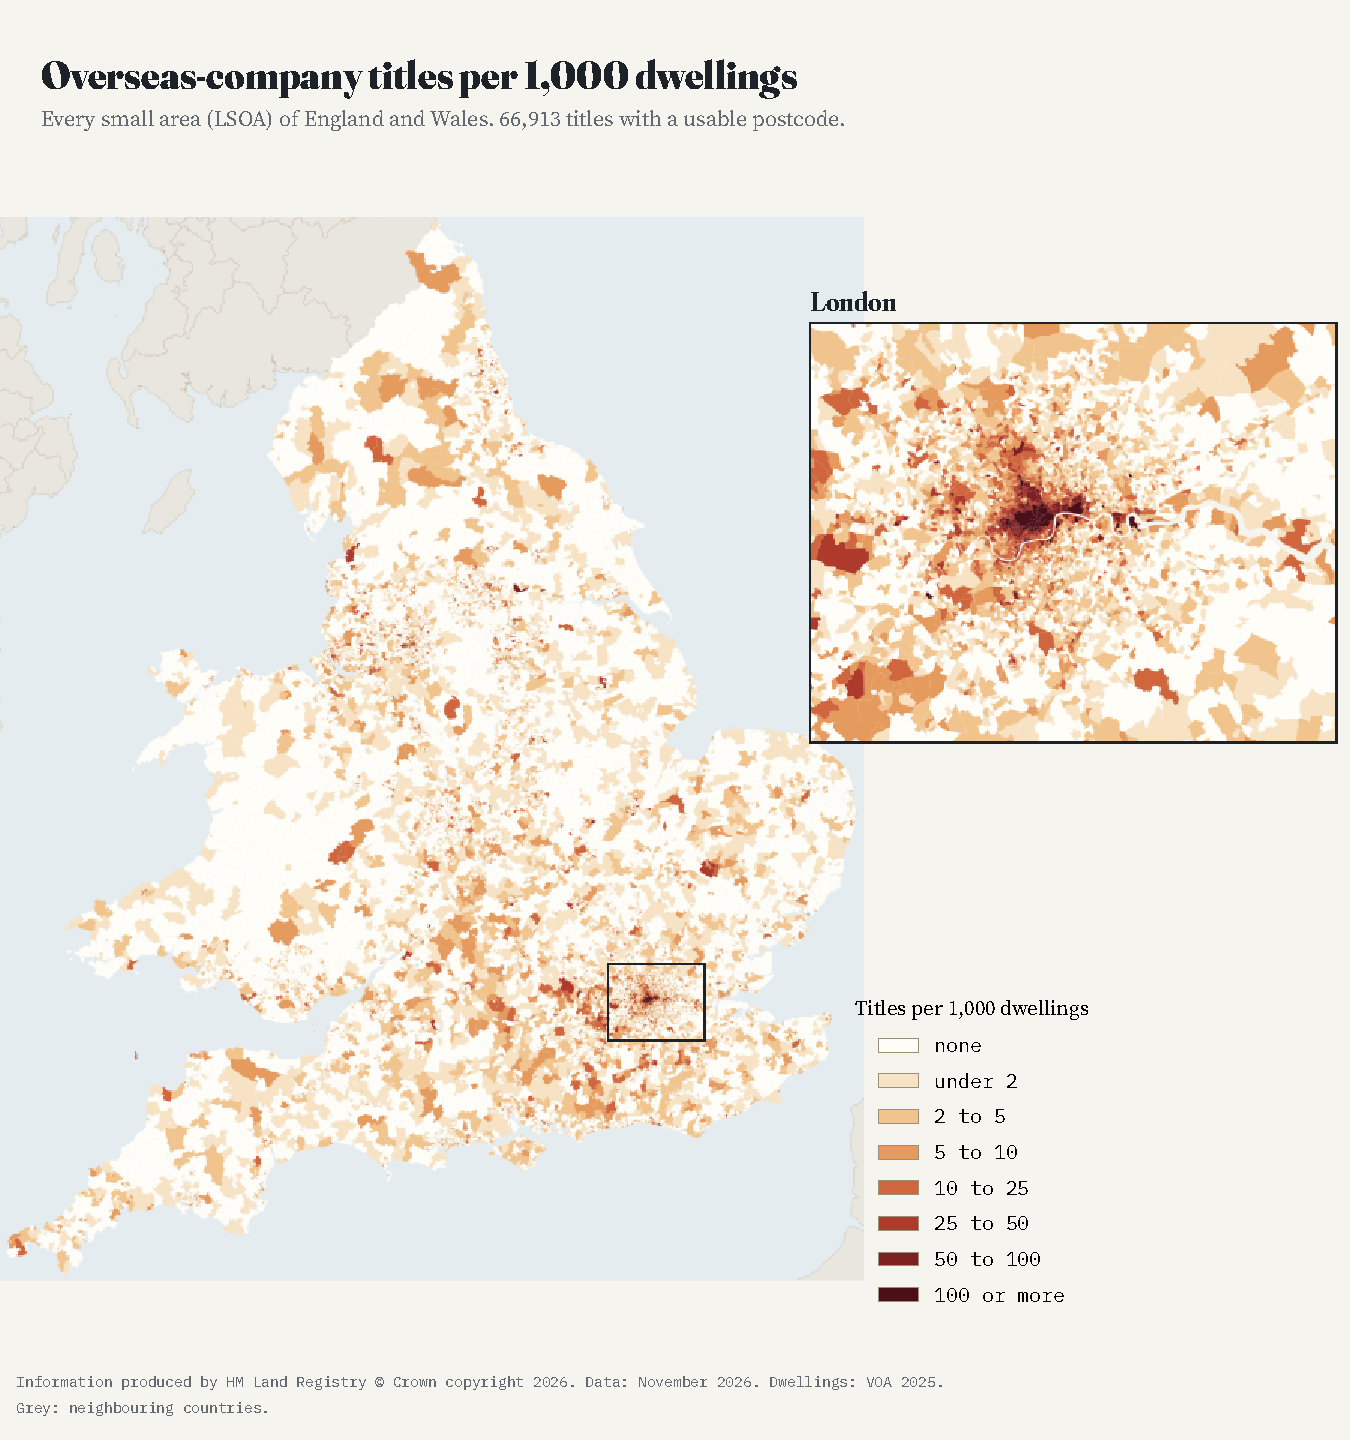
\includegraphics[width=0.95\textwidth]{f_map.pdf}
\caption{Overseas-company titles per 1,000 dwellings in each LSOA of England and Wales, November 2026 titles and March 2025 dwellings. 66,913 titles with a usable postcode; titles without one are counted only in district totals. Information produced by HM Land Registry \textcopyright{} Crown copyright 2026.}\label{fig:map}
\end{figure}

\begin{table}[tbp]\centering\small\caption{The 20 districts with the highest rates of overseas-company titles per 1,000 dwellings. UK-linked: share of titles held from the Crown Dependencies and Overseas Territories.}\label{tab:lad}\begin{tabular}{rllrrrr}\toprule & District & Region & Titles & Dwellings & Per 1,000 & UK-linked \%\\\midrule
1 & City of London & London & 1,412 & 8,060 & 175.2 & 44\\
2 & Westminster & London & 9,611 & 132,270 & 72.7 & 72\\
3 & Kensington and Chelsea & London & 4,914 & 89,310 & 55.0 & 76\\
4 & Camden & London & 2,040 & 114,020 & 17.9 & 71\\
5 & Tower Hamlets & London & 2,274 & 149,880 & 15.2 & 62\\
6 & Hammersmith and Fulham & London & 1,231 & 95,120 & 12.9 & 73\\
7 & Wandsworth & London & 1,957 & 157,960 & 12.4 & 79\\
8 & Lambeth & London & 1,732 & 148,670 & 11.7 & 42\\
9 & Hounslow & London & 1,157 & 111,350 & 10.4 & 32\\
10 & Southwark & London & 1,523 & 150,080 & 10.2 & 84\\
11 & Salford & North West & 1,368 & 135,790 & 10.1 & 85\\
12 & Islington & London & 1,076 & 112,240 & 9.6 & 66\\
13 & Colchester & East of England & 820 & 86,550 & 9.5 & 14\\
14 & Barnet & London & 1,057 & 160,580 & 6.6 & 72\\
15 & Hackney & London & 787 & 120,790 & 6.5 & 79\\
16 & North Warwickshire & West Midlands & 192 & 29,690 & 6.5 & 85\\
17 & St. Helens & North West & 555 & 86,200 & 6.4 & 97\\
18 & Manchester & North West & 1,603 & 252,920 & 6.3 & 75\\
19 & Ealing & London & 945 & 149,920 & 6.3 & 72\\
20 & Richmond upon Thames & London & 536 & 85,890 & 6.2 & 84\\
\bottomrule\end{tabular}\end{table}

At the small-area scale the concentration is sharper still (Figure~\ref{fig:conc}). The Gini coefficient of titles across LSOAs is 0.87, against 0.14 for dwellings. The 357 LSOAs with the most titles (the top 1\%) hold 39.2\% of geocoded titles and 1.6\% of dwellings, and half of all geocoded titles are in 744 LSOAs (2.1\%). At the same time the titles are widespread: 14,067 LSOAs (39.4\%) contain at least one. 41 LSOAs with at least 50 dwellings have 100 or more titles per 1,000 dwellings.

\begin{figure}[tbp]\centering
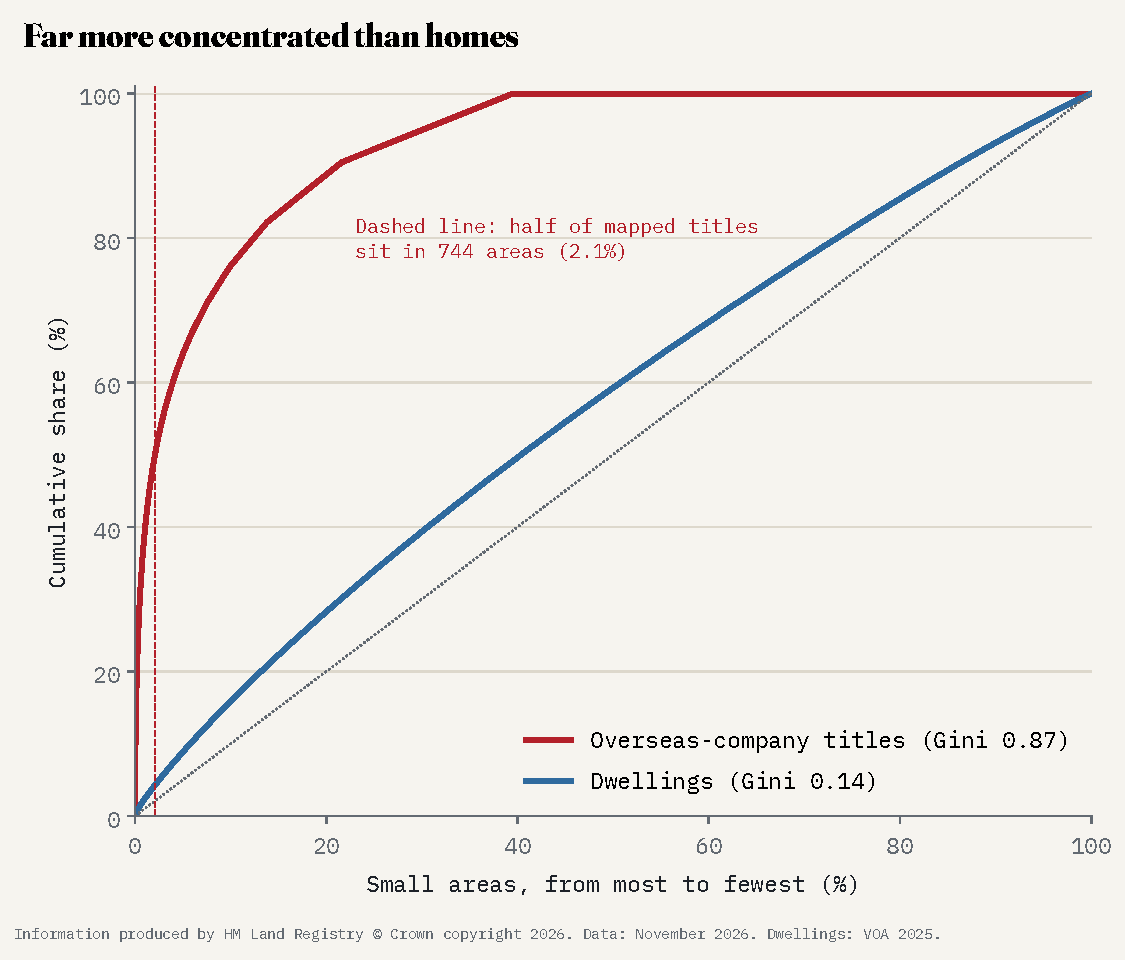
\includegraphics[width=0.62\textwidth]{f_conc.pdf}
\caption{Concentration curves across 35,672 LSOAs: cumulative share of overseas-company titles and of dwellings, areas ordered from most to fewest.}\label{fig:conc}
\end{figure}

H1 is supported on both pre-specified criteria. The titles Gini is far above the dwellings Gini, and Westminster and Kensington and Chelsea are second and third by rate. The expectation that they would be the two highest was wrong in detail: the City of London, with few homes and many commercial titles, ranks first.

\subsection{Which jurisdictions (H2)}
The companies are incorporated in 131 named jurisdictions, but four dominate (Figure~\ref{fig:jur}, Table~\ref{tab:jur}): Jersey (24,372 titles, 26.8\%), the British Virgin Islands (18,665, 20.5\%), Guernsey (12,216, 13.4\%) and the Isle of Man (9,632, 10.6\%). Together they hold 71.3\%. Companies from all the UK-linked offshore jurisdictions hold 68,812 titles, 75.7\%: 50.9\% from the Crown Dependencies and 24.7\% from the Overseas Territories. Counting a title for any of its proprietors makes almost no difference (75.7\%), since only 142 titles have proprietors from more than one jurisdiction. H2 is supported. Using the 2018 Financial Secrecy Index instead, 78.5\% of the titles whose jurisdiction has a score are held from jurisdictions with a secrecy score of 65 or more.

\begin{figure}[tbp]\centering
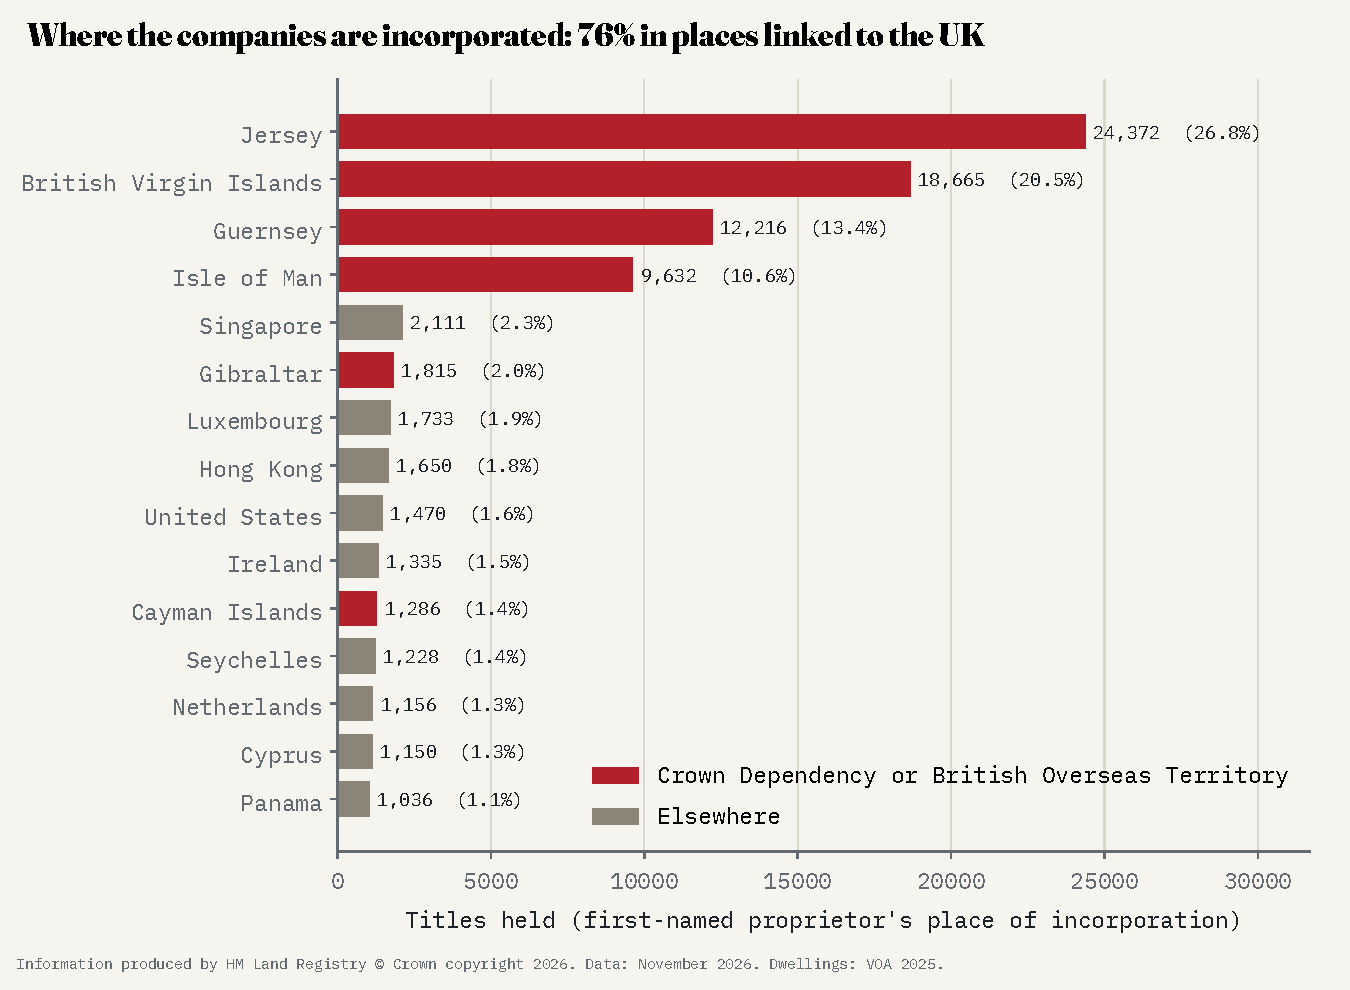
\includegraphics[width=0.82\textwidth]{f_jur.pdf}
\caption{Titles by the first proprietor's place of incorporation, 15 most common.}\label{fig:jur}
\end{figure}

\begin{table}[tbp]\centering\small\caption{The 15 most common jurisdictions of incorporation (first-named proprietor), with the 2018 Financial Secrecy Index secrecy score.}\label{tab:jur}\begin{tabular}{llrrr}\toprule Jurisdiction & UK link & Titles & \% & FSI 2018 score\\\midrule
Jersey & Crown Dependency & 24,372 & 26.8 & 65.5\\
British Virgin Islands & Overseas Territory & 18,665 & 20.5 & 68.7\\
Guernsey & Crown Dependency & 12,216 & 13.4 & 72.5\\
Isle of Man & Crown Dependency & 9,632 & 10.6 & 63.6\\
Singapore &  & 2,111 & 2.3 & 67.1\\
Gibraltar & Overseas Territory & 1,815 & 2.0 & 70.8\\
Luxembourg &  & 1,733 & 1.9 & 58.2\\
Hong Kong &  & 1,650 & 1.8 & 71.0\\
United States &  & 1,470 & 1.6 & 59.8\\
Ireland &  & 1,335 & 1.5 & 50.6\\
Cayman Islands & Overseas Territory & 1,286 & 1.4 & 72.3\\
Seychelles &  & 1,228 & 1.4 & 75.2\\
Netherlands &  & 1,156 & 1.3 & 66.0\\
Cyprus &  & 1,150 & 1.3 & 61.2\\
Panama &  & 1,036 & 1.1 & 76.6\\
\midrule All Crown Dependencies and Overseas Territories & & 68,812 & 75.7 & \\
\bottomrule\end{tabular}\end{table}

The share held from UK-linked jurisdictions is lower in London (70.0\%) than in any other region, and highest in Wales (85.5\%; Appendix Table~\ref{tab:region}). In London a wider range of jurisdictions appears, including Singapore, Hong Kong, Luxembourg and the Netherlands.

\subsection{What kind of small area (H3)}
Table~\ref{tab:main} reports the main model. Within the same district, an LSOA with 10 percentage points more of its dwellings in the top Council Tax bands has 29\% more overseas-company titles per dwelling (rate ratio 1.293, 95\% CI 1.226 to 1.363); 10 points more flats goes with 30\% more titles (1.298, 1.272 to 1.325); and 10 points more homes built since 2009 with 9.8\% more (1.098, 1.060 to 1.136). All three components of H3 are supported. The three shares are only weakly correlated across LSOAs (the largest correlation, between flats and new homes, is 0.20), and the univariate estimates are similar except for new-build, whose association roughly halves once flats are held constant.

\begin{table}[tbp]\centering\footnotesize\caption{Overseas-company titles per dwelling and the housing stock of the LSOA: incidence rate ratios per 10 percentage points [95\% CI]. PPML with district fixed effects (district by jurisdiction group in the interaction model), offset log dwellings, standard errors clustered by district. Univariate: each share alone. UK-linked and Elsewhere: titles from those jurisdiction groups only. Interaction: ratio of the UK-linked to the Elsewhere gradient in a stacked model. Districts with no titles in a group drop out of that model.}\label{tab:main}\resizebox{\textwidth}{!}{\begin{tabular}{lccccc}\toprule & Main & Univariate & UK-linked & Elsewhere & Interaction\\\midrule
Top Council Tax bands (per 10 points) & 1.293 [1.226, 1.363] & 1.213 [1.141, 1.289] & 1.268 [1.199, 1.342] & 1.370 [1.276, 1.471] & 0.926 [0.864, 0.992]\\
Flats and maisonettes (per 10 points) & 1.298 [1.272, 1.325] & 1.295 [1.254, 1.338] & 1.276 [1.252, 1.300] & 1.385 [1.307, 1.467] & 0.921 [0.868, 0.979]\\
Built 2009 or later (per 10 points) & 1.098 [1.060, 1.136] & 1.229 [1.191, 1.269] & 1.109 [1.067, 1.151] & 1.059 [1.015, 1.104] & 1.047 [1.000, 1.096]\\
N (LSOAs) & 35,672 & 35,672 & 35,672 & 35,607 & 71,279\\
Districts (clusters) & 318 & 318 & 318 & 316 & 318\\
\bottomrule\end{tabular}}\end{table}

The jurisdiction groups differ in degree, not direction (H3s). For titles from the UK-linked offshore jurisdictions the rate ratios are 1.27, 1.28 and 1.11; for titles from everywhere else they are 1.37, 1.38 and 1.06. In the stacked model, the gradients with the top-band share and the flat share are somewhat flatter for the UK-linked group (interaction rate ratios 0.93 and 0.92), and the new-build gradient slightly steeper (1.05, with a confidence interval that just excludes 1).

\subsection{When the current owners were added}
Figure~\ref{fig:years} shows the titles by the year the current proprietor was added. Only 2,916 current titles have an owner added before 2000. The count rises through the 2000s and 2010s to a peak in 2017 (6,544 titles), and is lower from 2020: an average of 3,718 a year in 2022 to 2025 against 5,707 in 2015 to 2019. Because titles sold on leave the file, the older years are understated and the profile cannot be read as a series of purchases. The share from the UK-linked offshore jurisdictions is similar across periods: 73\% for owners added 1999 to 2009, 79\% for 2017 to 2021 and 77\% since 2022. This snapshot design cannot test the effect of the 2022 register; \citet{collin2025} use repeated files for that purpose.

\begin{figure}[tbp]\centering
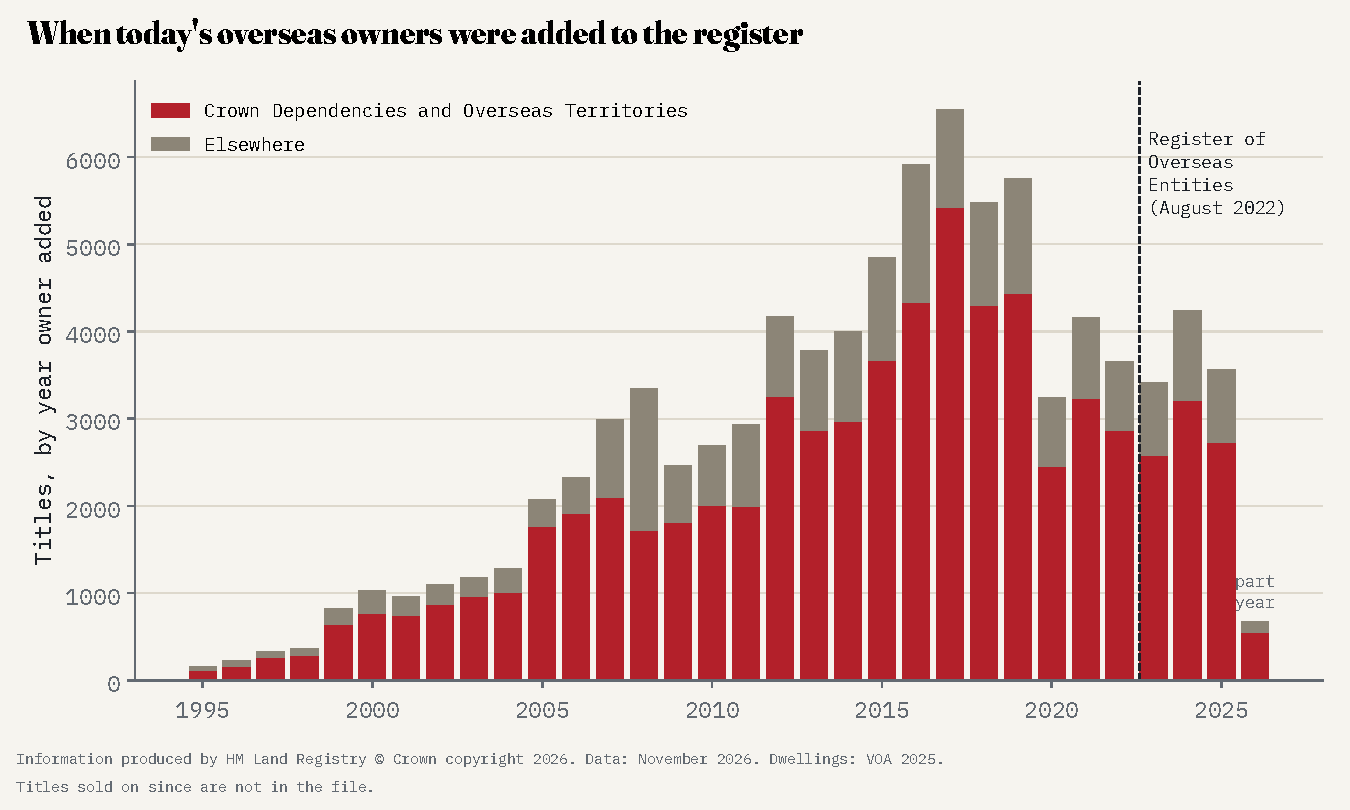
\includegraphics[width=0.85\textwidth]{f_years.pdf}
\caption{Titles in the November 2026 file by the year the current proprietor was added. 2026 is a part year. Titles sold since are not in the file.}\label{fig:years}
\end{figure}

\subsection{Prices and holders}
Price paid is recorded for 34,127 titles. Its median is \pounds{}500,000 (quartiles \pounds{}205,000 and \pounds{}1,686,742); 34\% are £1 million or more. The median is higher for titles from the UK-linked offshore jurisdictions (\pounds{}530,347) than for others (\pounds{}435,000), higher for freeholds (\pounds{}800,000) than leaseholds (\pounds{}402,000), and much higher in London (\pounds{}715,000) than elsewhere (\pounds{}287,500) (Appendix Figure~\ref{fig:price}). These are prices at registration over three decades and are not adjusted for inflation or comparable across property types.

Most proprietors hold few titles. Of 28,198 distinct first-named proprietors, 63\% hold a single title. A small number of portfolios still matter: the ten largest hold 8.7\% of titles and the 66 proprietors with 100 or more titles hold 19.8\% (Figure~\ref{fig:holders}). Several of the largest hold titles in more than 100 districts; one holds 1,193 titles in 2 districts. Counting titles is not counting value, and a large count says nothing about the conduct of the company.

\begin{figure}[tbp]\centering
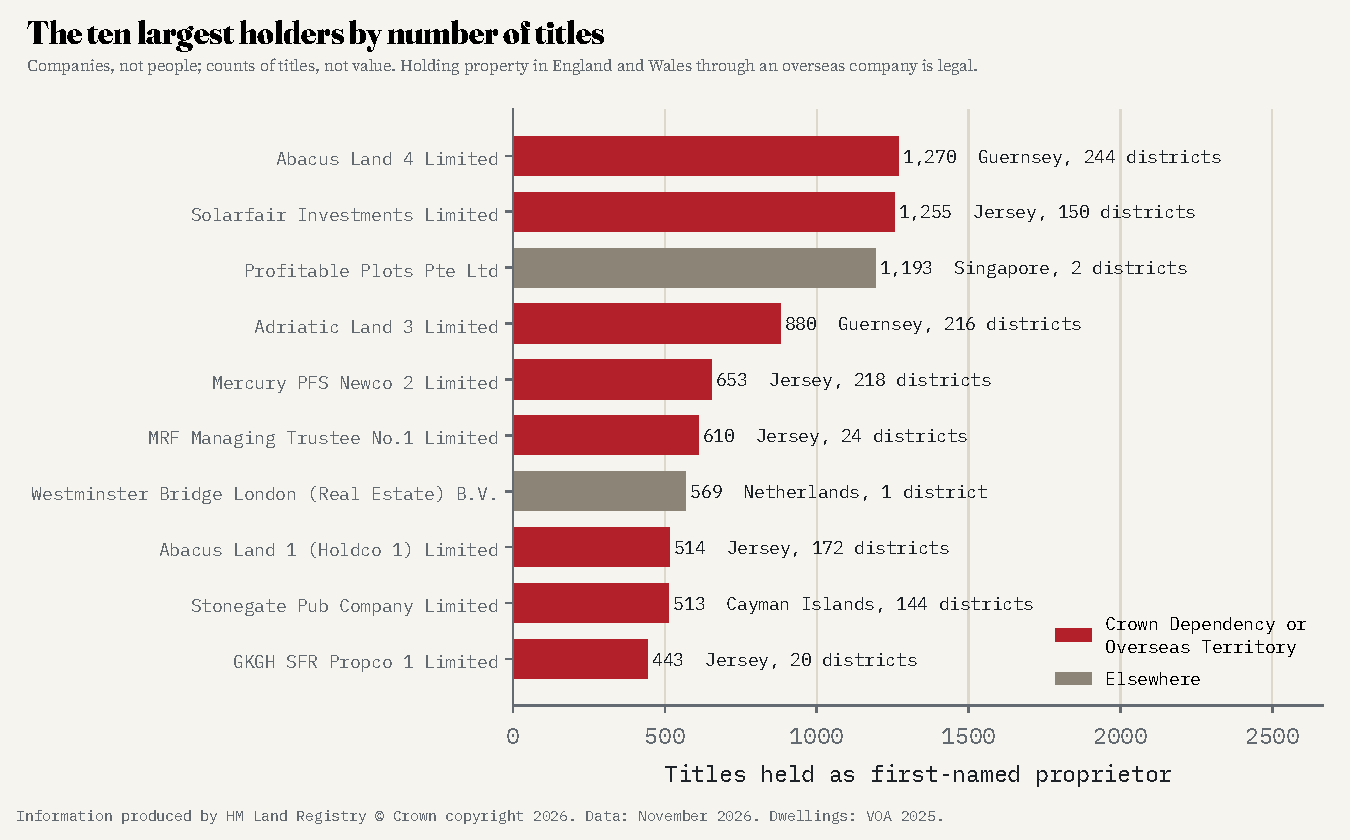
\includegraphics[width=0.85\textwidth]{f_holders.pdf}
\caption{The ten largest first-named proprietors by number of titles, with jurisdiction and number of districts. Holding property in England and Wales through an overseas company is legal.}\label{fig:holders}
\end{figure}

\section{Robustness}\label{sec:robust}
Figure~\ref{fig:models} and Table~\ref{tab:robust} report the planned checks. In every one of the 18 alternative models all three rate ratios stay above 1 with confidence intervals that exclude 1. The negative binomial model (dispersion 1.87) gives 1.19, 1.27 and 1.13. Leaving out London matters most for the top-band share, which falls to 1.16: part of the prime-market gradient is a London phenomenon, but it remains outside London. Leaving out any other region changes little (the top-band rate ratio ranges from 1.16 to 1.30 across the ten leave-one-region-out models). Dropping Westminster and Kensington and Chelsea gives 1.23, 1.30 and 1.11.

The measurement checks behave as expected if the pattern reflects residential investment. Restricting to residential-looking titles strengthens all three associations (1.40, 1.56, 1.15), as does restricting to leaseholds, while freeholds, which include land and commercial property, show weaker but still positive associations. Single-address titles and the alternative treatment of suppressed VOA cells leave the estimates unchanged to two decimal places. With region instead of district fixed effects the top-band and flat ratios are larger (1.38 and 1.36), showing that part of the cross-district pattern is absorbed by the within-district design.

In the placebo, each district's titles were reallocated at random across its LSOAs in proportion to dwellings, 200 times. The placebo rate ratios centre on 1 (1.000, 1.000 and 1.000), with 95\% of draws between 0.995 and 1.004 for the top-band share and similarly narrow ranges for the others. None of the 200 draws comes close to the observed estimates. The associations are therefore not a mechanical product of the offset, the district effects or the distribution of dwellings.

\begin{figure}[tbp]\centering
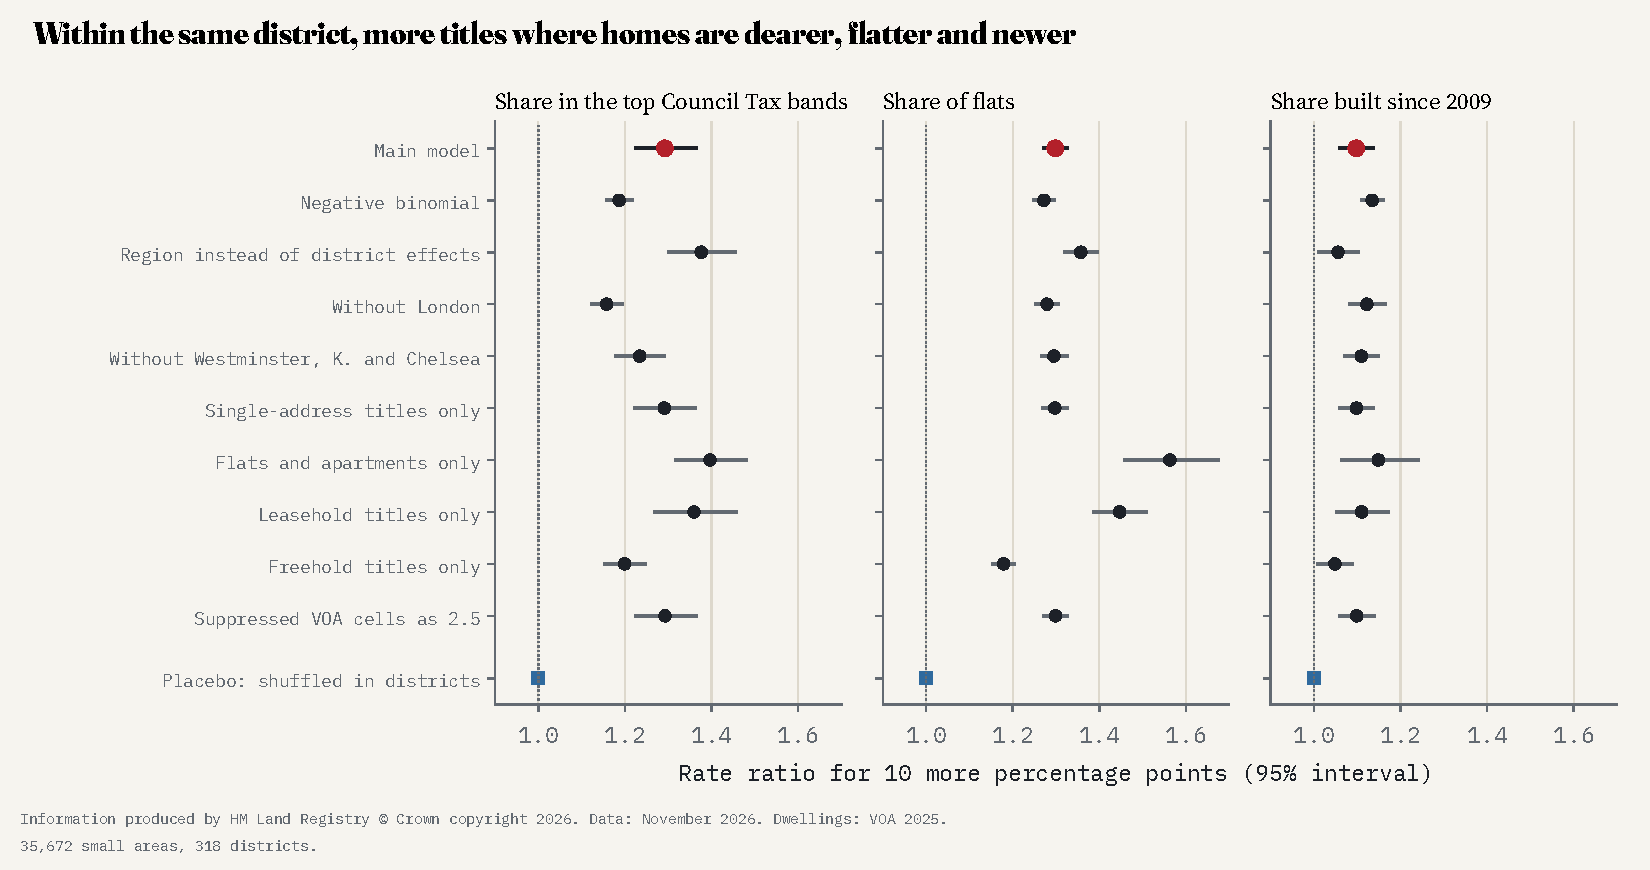
\includegraphics[width=\textwidth]{f_models.pdf}
\caption{Rate ratios per 10 percentage points with 95\% confidence intervals, main model and planned checks, and the placebo (95\% range of 200 draws).}\label{fig:models}
\end{figure}

\begin{table}[tbp]\centering\footnotesize\caption{Robustness: incidence rate ratios per 10 percentage points [95\% CI] under each planned check.}\label{tab:robust}\resizebox{\textwidth}{!}{\begin{tabular}{lcccr}\toprule Check & Top bands & Flats & Built 2009 or later & N\\\midrule
Main model & 1.29 [1.23, 1.36] & 1.30 [1.27, 1.32] & 1.10 [1.06, 1.14] & 35,672\\\midrule
Region instead of district fixed effects & 1.38 [1.30, 1.45] & 1.36 [1.32, 1.39] & 1.06 [1.01, 1.10] & 35,672\\
Negative binomial (NB2), district fixed effects & 1.19 [1.16, 1.22] & 1.27 [1.25, 1.29] & 1.13 [1.11, 1.16] & 35,672\\
Without East Midlands & 1.30 [1.23, 1.37] & 1.30 [1.27, 1.33] & 1.10 [1.06, 1.14] & 32,825\\
Without East of England & 1.30 [1.23, 1.37] & 1.30 [1.27, 1.33] & 1.09 [1.05, 1.13] & 31,914\\
Without London & 1.16 [1.12, 1.19] & 1.28 [1.25, 1.30] & 1.12 [1.08, 1.16] & 30,678\\
Without North East & 1.29 [1.23, 1.36] & 1.30 [1.27, 1.32] & 1.10 [1.06, 1.14] & 33,990\\
Without North West & 1.30 [1.24, 1.37] & 1.30 [1.27, 1.33] & 1.09 [1.06, 1.13] & 31,105\\
Without South East & 1.30 [1.22, 1.38] & 1.30 [1.27, 1.33] & 1.10 [1.06, 1.14] & 30,101\\
Without South West & 1.30 [1.23, 1.37] & 1.31 [1.28, 1.33] & 1.10 [1.06, 1.14] & 32,265\\
Without Wales & 1.29 [1.23, 1.37] & 1.30 [1.27, 1.33] & 1.10 [1.06, 1.14] & 33,755\\
Without West Midlands & 1.30 [1.23, 1.37] & 1.30 [1.27, 1.32] & 1.10 [1.06, 1.14] & 32,098\\
Without Yorkshire and The Humber & 1.30 [1.23, 1.37] & 1.29 [1.27, 1.32] & 1.10 [1.06, 1.14] & 32,317\\
Without Westminster and Kensington and Chelsea & 1.23 [1.18, 1.29] & 1.30 [1.27, 1.32] & 1.11 [1.07, 1.15] & 35,448\\
Single-address titles only & 1.29 [1.22, 1.36] & 1.30 [1.27, 1.32] & 1.10 [1.06, 1.14] & 35,672\\
Residential-looking titles only & 1.40 [1.32, 1.48] & 1.56 [1.46, 1.67] & 1.15 [1.06, 1.24] & 29,313\\
Leasehold titles only & 1.36 [1.27, 1.46] & 1.45 [1.39, 1.51] & 1.11 [1.05, 1.17] & 35,603\\
Freehold titles only & 1.20 [1.15, 1.25] & 1.18 [1.16, 1.20] & 1.05 [1.01, 1.09] & 35,672\\
VOA suppressed cells as 2.5 & 1.29 [1.22, 1.36] & 1.30 [1.27, 1.33] & 1.10 [1.06, 1.14] & 35,672\\
\midrule Placebo: mean [2.5th, 97.5th percentile] of 200 draws & 1.000 [0.995, 1.004] & 1.000 [0.995, 1.004] & 1.000 [0.995, 1.006] & 35,672\\
\bottomrule\end{tabular}}\end{table}

\section{Exploratory analysis}\label{sec:explore}
After seeing the planned results I looked at the small areas with the highest rates. Several are single buildings or developments in which many units are registered as separate titles to the same company. In 4 of the 10 LSOAs with the highest rates one proprietor holds more than half the titles. Across England and Wales, 7,573 geocoded titles (11.3\%) are in blocks of 20 or more held by one proprietor in one LSOA, spread over 144 LSOAs. This is one reason why the very highest small-area rates should be read with care, and why the district and regression results, which average over many areas, are a better guide than any single hot spot.

\section{Discussion}\label{sec:disc}
\subsection{What the pattern says}
The register describes a stock of property that is at once highly concentrated and widely spread. A few central London districts hold a share of titles about 20 times their share of homes, and the top 1\% of small areas hold 24 times their share. Yet 39\% of small areas have at least one title, and every district has some. Most of the register is not in prime London: 57\% of titles are outside the capital.

The UK's own offshore jurisdictions dominate the register, and more so outside London than inside it. This is consistent with the account of a British-centred offshore network in \citet{haberly2015a} and \citet{palan2010}, and the largest holders show that Crown Dependency companies are used for large portfolios as well as for single properties: 6 of the ten largest hold titles in more than 100 districts each. The higher UK-linked share outside London is consistent with such portfolios making up a substantial part of the register there, alongside the individual high-value purchases that dominate public discussion, although the register cannot measure this directly. The register cannot separate these uses, and a jurisdiction is not evidence of secrecy or wrongdoing: many companies in these places are ordinary investment vehicles with disclosed owners, and since 2022 their beneficial owners must be declared to Companies House.

Within districts, overseas-company titles favour higher-band, flatted and newer neighbourhoods. The flat gradient is the strongest and most stable, and it strengthens when the outcome is restricted to residential-looking titles. That is consistent with the idea that the investment product sold to overseas companies is often the flat in a new or recent block \citep{tiuk2017,bourne2022}. The top-band gradient is partly a London effect, consistent with the literature on prime London \citep{webber2016,burrows2017}, but it is present outside London too.

\subsection{Limitations}
Five limitations matter. First, the register records legal owners incorporated overseas. Property owned from abroad through UK companies, trusts or in an individual's name is not in it, and neither is property owned by overseas companies through UK subsidiaries. The register is therefore a lower bound on foreign or offshore interest in property. Second, titles are not dwellings, and their scale varies from a parking space to a business park. The rate per dwelling is a convenient normalisation, not a share of homes owned. Third, the file is a snapshot. It shows who holds titles in November 2026, and the year the owner was added; it cannot show turnover or the history of titles sold on. Fourth, about a quarter of titles have no usable postcode and enter only district totals; if these differ systematically from the geocoded titles (they are more often land), the small-area results describe the geocoded part of the register. Fifth, the neighbourhood measures are crude. Council Tax bands reflect values in 1991 in England and 2003 in Wales; the flat and new-build shares describe the stock, not the titles themselves. All results are associations; none is an effect of one variable on another.

\subsection{Implications}
For research, the aggregates published with this paper make it possible to use the register at small-area scale without handling title-level data, which the licence restricts. They can be joined to other small-area data on vacancy, prices, deprivation or local politics. For public debate, the results suggest that the overseas-company register is both more London-centred and more widespread than either headline totals or prime-London case studies convey, and that most of it is held through vehicles in the UK's own Crown Dependencies and Overseas Territories.

\section{Conclusion}\label{sec:conc}
Using the full HM Land Registry file of property titles held by overseas companies, this paper maps the register for every small area of England and Wales and relates it to the housing stock. The titles are extremely concentrated in central London but present in 39\% of small areas; 76\% are held through companies from the UK's Crown Dependencies and Overseas Territories; and within districts they are more common where homes are in higher Council Tax bands, are flats, and are newer. Each result was specified in advance and survives every planned check. What the register cannot show, who stands behind these companies and why they hold property where they do, needs the beneficial ownership data that the 2022 reforms have begun to create.

\section*{Data availability statement}
Data and code: Zenodo DOI https://doi.org/10.5281/zenodo.24115198. The archive contains the aggregate counts by small area, district, region, jurisdiction, year and price group, the model estimates and all code. It does not contain the HM Land Registry title-level file, which is available from HM Land Registry under its own licence; the code reproduces every result from that file. Information produced by HM Land Registry \textcopyright{} Crown copyright 2026.

\section*{AI statement}
I wrote the text, with drafting and editing assistance from Claude (Anthropic), which also helped prepare the analysis code. I reviewed and checked all text and results.

\begin{thebibliography}{99}
\bibitem[Aalbers(2016)]{aalbers2016} Aalbers, M. B. (2016) \textit{The Financialization of Housing: A Political Economy Approach}. Abingdon: Routledge.
\bibitem[Abadie et al.(2023)]{abadie2023} Abadie, A., Athey, S., Imbens, G. W. and Wooldridge, J. M. (2023) When should you adjust standard errors for clustering? \textit{Quarterly Journal of Economics} 138(1), 1 to 35. doi:10.1093/qje/qjac038.
\bibitem[Alstads{\ae}ter et al.(2018)]{alstadsaeter2018} Alstads{\ae}ter, A., Johannesen, N. and Zucman, G. (2018) Who owns the wealth in tax havens? Macro evidence and implications for global inequality. \textit{Journal of Public Economics} 162, 89 to 100.
\bibitem[Atkinson(2020)]{atkinson2020} Atkinson, R. (2020) \textit{Alpha City: How London Was Captured by the Super-Rich}. London: Verso.
\bibitem[Atkinson et al.(2017)]{atkinson2017} Atkinson, R., Burrows, R., Glucksberg, L., Ho, H. K., Knowles, C. and Rhodes, D. (2017) Minimum city? The deeper impacts of the `super-rich' on urban life. In Forrest, R., Koh, S. Y. and Wissink, B. (eds) \textit{Cities and the Super-Rich: Real Estate, Elite Practices and Urban Political Economies}. New York: Palgrave Macmillan. doi:10.1057/978-1-137-54834-4\_13.
\bibitem[Badarinza and Ramadorai(2018)]{badarinza2018} Badarinza, C. and Ramadorai, T. (2018) Home away from home? Foreign demand and London house prices. \textit{Journal of Financial Economics} 130(3), 532 to 555.
\bibitem[Bomare and Le Guern Herry(2022)]{bomare2022} Bomare, J. and Le Guern Herry, S. (2022) Will we ever be able to track offshore wealth? Evidence from the offshore real estate market in the UK. EU Tax Observatory Working Paper 4.
\bibitem[Bourne et al.(2023)]{bourne2022} Bourne, J., Ingianni, A. and McKenzie, R. (2023) What's in the laundromat? Mapping and characterising offshore-owned residential property in London. \textit{Environment and Planning B: Urban Analytics and City Science} 50(9), 2430 to 2451. doi:10.1177/23998083231155483.
\bibitem[Burrows et al.(2017)]{burrows2017} Burrows, R., Webber, R. and Atkinson, R. (2017) Welcome to `Pikettyville'? Mapping London's alpha territories. \textit{The Sociological Review} 65(2), 184 to 201. doi:10.1111/1467-954X.12375.
\bibitem[Cameron and Miller(2015)]{cameron2015} Cameron, A. C. and Miller, D. L. (2015) A practitioner's guide to cluster-robust inference. \textit{Journal of Human Resources} 50(2), 317 to 372.
\bibitem[Cobham et al.(2015)]{cobham2015} Cobham, A., Jansk\'y, P. and Meinzer, M. (2015) The Financial Secrecy Index: shedding new light on the geography of secrecy. \textit{Economic Geography} 91(3), 281 to 303.
\bibitem[Collin et al.(2025)]{collin2025} Collin, M., Hollenbach, F. M. and Szakonyi, D. (2025) The end of Londongrad? Ownership transparency and offshore investment in real estate. EU Tax Observatory Working Paper 28.
\bibitem[Correia et al.(2020)]{correia2020} Correia, S., Guimar\~aes, P. and Zylkin, T. (2020) Fast Poisson estimation with high-dimensional fixed effects. \textit{Stata Journal} 20(1), 95 to 115. doi:10.1177/1536867X20909691.
\bibitem[Economic Crime Act(2022)]{ecta2022} Economic Crime (Transparency and Enforcement) Act 2022, c. 10. London: The Stationery Office. Part 1 (Register of Overseas Entities) in force from 1 August 2022.
\bibitem[Fernandez et al.(2016)]{fernandez2016} Fernandez, R., Hofman, A. and Aalbers, M. B. (2016) London and New York as a safe deposit box for the transnational wealth elite. \textit{Environment and Planning A} 48(12), 2443 to 2461. doi:10.1177/0308518X16659479.
\bibitem[Garcia-Bernardo et al.(2017)]{garcia2017} Garcia-Bernardo, J., Fichtner, J., Takes, F. W. and Heemskerk, E. M. (2017) Uncovering offshore financial centers: conduits and sinks in the global corporate ownership network. \textit{Scientific Reports} 7, 6246. doi:10.1038/s41598-017-06322-9.
\bibitem[Gorback and Keys(2020)]{gorback2020} Gorback, C. S. and Keys, B. J. (2020) Global capital and local assets: house prices, quantities, and elasticities. NBER Working Paper 27370.
\bibitem[Haberly and W\'ojcik(2015a)]{haberly2015a} Haberly, D. and W\'ojcik, D. (2015a) Regional blocks and imperial legacies: mapping the global offshore FDI network. \textit{Economic Geography} 91(3), 251 to 280.
\bibitem[Haberly and W\'ojcik(2015b)]{haberly2015b} Haberly, D. and W\'ojcik, D. (2015b) Tax havens and the production of offshore FDI: an empirical analysis. \textit{Journal of Economic Geography} 15(1), 75 to 101.
\bibitem[Harrington(2016)]{harrington2016} Harrington, B. (2016) \textit{Capital without Borders: Wealth Managers and the One Percent}. Cambridge, MA: Harvard University Press.
\bibitem[HM Land Registry(2026)]{hmlr2026} HM Land Registry (2026) Overseas companies that own property in England and Wales, full file, November 2026. Use land and property data service. Information produced by HM Land Registry \textcopyright{} Crown copyright 2026; used under HM Land Registry's licence for this dataset.
\bibitem[Johannesen and Zucman(2014)]{johannesen2014} Johannesen, N. and Zucman, G. (2014) The end of bank secrecy? An evaluation of the G20 tax haven crackdown. \textit{American Economic Journal: Economic Policy} 6(1), 65 to 91. doi:10.1257/pol.6.1.65.
\bibitem[Knowles(2022)]{knowles2022} Knowles, C. (2022) \textit{Serious Money: Walking Plutocratic London}. London: Allen Lane.
\bibitem[Ley(2017)]{ley2017} Ley, D. (2017) Global China and the making of Vancouver's residential property market. \textit{International Journal of Housing Policy} 17(1), 15 to 34.
\bibitem[ONS(2021)]{ons2021lsoa} Office for National Statistics (2021) Lower layer Super Output Areas (December 2021) boundaries EW BGC; Local Authority Districts (December 2023) boundaries UK BGC. Open Government Licence v3.0. LSOAs via github.com/drkane/geo-lookups, commit e20a072.
\bibitem[Palan et al.(2010)]{palan2010} Palan, R., Murphy, R. and Chavagneux, C. (2010) \textit{Tax Havens: How Globalization Really Works}. Ithaca, NY: Cornell University Press.
\bibitem[Rogers and Koh(2017)]{rogers2017} Rogers, D. and Koh, S. Y. (2017) The globalisation of real estate: the politics and practice of foreign real estate investment. \textit{International Journal of Housing Policy} 17(1), 1 to 14.
\bibitem[S\'a(2025)]{sa2025} S\'a, F. (2025) The effect of foreign investors on local housing markets: evidence from the UK. \textit{Journal of Economic Geography} 25(3), 329 to 349. doi:10.1093/jeg/lbae043.
\bibitem[Santos Silva and Tenreyro(2006)]{santos2006} Santos Silva, J. M. C. and Tenreyro, S. (2006) The log of gravity. \textit{Review of Economics and Statistics} 88(4), 641 to 658. doi:10.1162/rest.88.4.641.
\bibitem[Shaxson(2011)]{shaxson2011} Shaxson, N. (2011) \textit{Treasure Islands: Tax Havens and the Men Who Stole the World}. London: Bodley Head.
\bibitem[Tax Justice Network(2018)]{tjn2018} Tax Justice Network (2018) \textit{Financial Secrecy Index 2018}. Secrecy scores as republished in github.com/Global-Witness/secret-property-analysis-2019-public (data/processed/financial\_secrecy\_index\_2018.csv).
\bibitem[Transparency International UK(2015)]{tiuk2015} Transparency International UK (2015) \textit{Corruption on Your Doorstep: How Corrupt Capital Is Used to Buy Property in the UK}. London: Transparency International UK.
\bibitem[Transparency International UK(2017)]{tiuk2017} Transparency International UK (2017) \textit{Faulty Towers: Understanding the Impact of Overseas Corruption on the London Property Market}. London: Transparency International UK.
\bibitem[VOA(2025)]{voa2025} Valuation Office Agency (2025) \textit{Council Tax: Stock of Properties, 2025}, tables CTSOP3.1 and CTSOP4.1. Official Statistics. Open Government Licence v3.0.
\bibitem[Webber and Burrows(2016)]{webber2016} Webber, R. and Burrows, R. (2016) Life in an alpha territory: discontinuity and conflict in an elite London `village'. \textit{Urban Studies} 53(15), 3139 to 3154.
\bibitem[Wetzstein(2017)]{wetzstein2017} Wetzstein, S. (2017) The global urban housing affordability crisis. \textit{Urban Studies} 54(14), 3159 to 3177.
\bibitem[Zucman(2013)]{zucman2013} Zucman, G. (2013) The missing wealth of nations: are Europe and the U.S. net debtors or net creditors? \textit{Quarterly Journal of Economics} 128(3), 1321 to 1364.
\end{thebibliography}

\appendix
\section{Appendix: further tables and data construction}\label{sec:appx}
\begin{table}[htbp]\centering\small\caption{Titles by region (all titles, including those placed by district only).}\label{tab:region}\begin{tabular}{lrrrrrr}\toprule Region & Titles & \% & Dwellings & Per 1,000 & UK-linked \% & Median price (\pounds)\\\midrule
London & 38,955 & 42.8 & 3,840,040 & 10.14 & 70.0 & 715,000\\
North West & 10,774 & 11.8 & 3,468,280 & 3.11 & 81.8 & 198,000\\
South East & 10,844 & 11.9 & 4,172,540 & 2.60 & 79.7 & 510,992\\
East of England & 6,730 & 7.4 & 2,865,130 & 2.35 & 72.0 & 334,110\\
Yorkshire and The Humber & 5,421 & 6.0 & 2,548,630 & 2.13 & 81.2 & 189,438\\
South West & 5,065 & 5.6 & 2,706,110 & 1.87 & 79.0 & 416,400\\
East Midlands & 4,134 & 4.5 & 2,234,870 & 1.85 & 80.5 & 243,945\\
West Midlands & 4,586 & 5.0 & 2,638,800 & 1.74 & 82.7 & 425,000\\
North East & 2,228 & 2.5 & 1,288,520 & 1.73 & 82.7 & 184,500\\
Wales & 2,212 & 2.4 & 1,485,150 & 1.49 & 85.5 & 256,212\\
\bottomrule\end{tabular}\end{table}

\begin{figure}[htbp]\centering
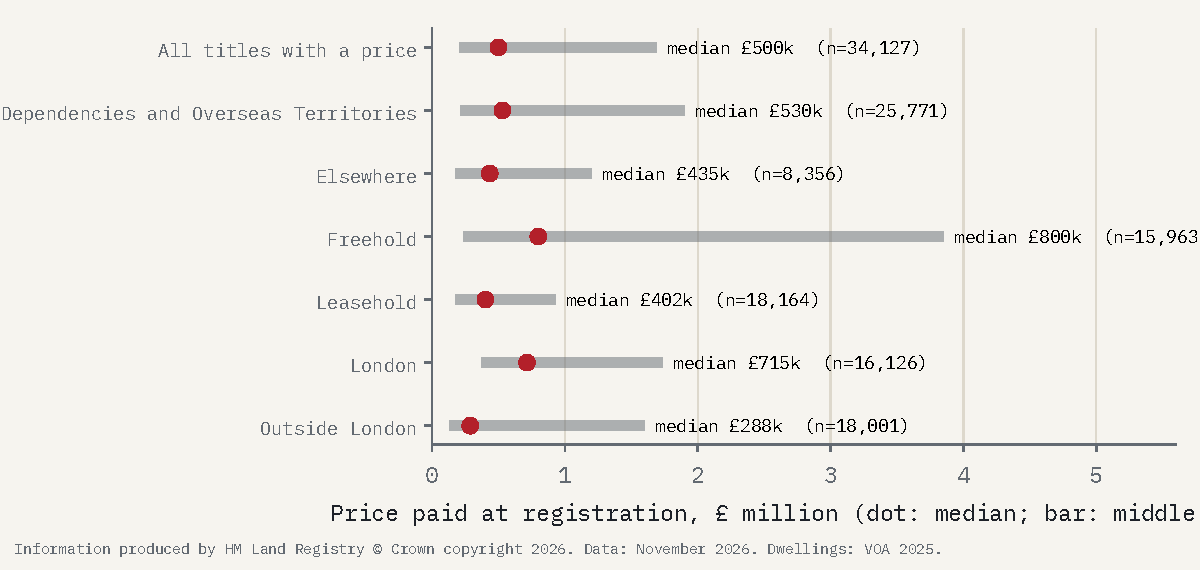
\includegraphics[width=0.8\textwidth]{f_price.pdf}
\caption{Price paid at registration where recorded: median and middle half, by group.}\label{fig:price}
\end{figure}

\begin{figure}[htbp]\centering
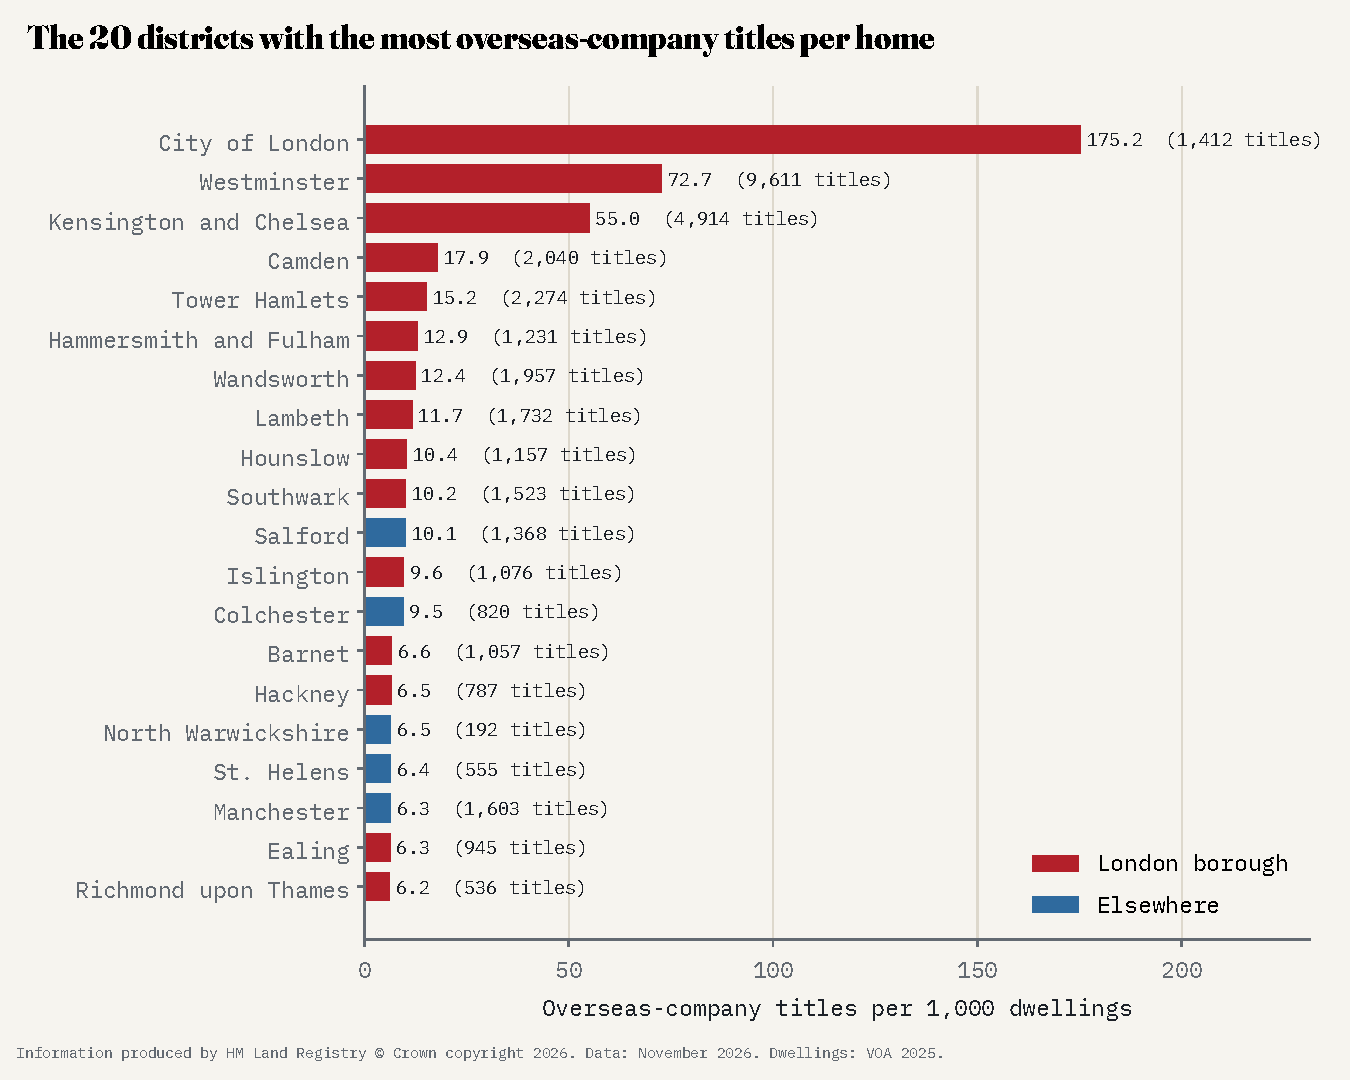
\includegraphics[width=0.85\textwidth]{f_lad.pdf}
\caption{The 20 districts with the highest rates of overseas-company titles per 1,000 dwellings (all titles, including those without a postcode).}\label{fig:lad}
\end{figure}

\textbf{Data construction.} (1) The OCOD file is read from the zip as text; the one row without tenure is dropped. (2) Postcodes are normalised (upper case, spaces removed) and matched to the postcodes.io geocodes; the LSOA's district comes from the ONS LSOA file (current district codes). (3) Titles without a matched postcode take the district in which geocoded titles with the same \texttt{District} value most often fall. (4) Country of incorporation is cleaned with a fixed table (code/common.py). (5) VOA LSOA rows are read from CTSOP4.1 (all bands; band rows; build periods) and CTSOP3.1 (flats and maisonettes); `-' is read as 0 (main) or 2.5 (check). (6) The PPML estimator concentrates out the district effects in closed form; it reproduces a statsmodels GLM with district dummies to $10^{-5}$. The negative binomial uses iteratively reweighted least squares with weighted within-district demeaning and a profile likelihood grid for the dispersion. (7) The placebo draws each district's total from a multinomial distribution over its LSOAs with probabilities proportional to dwellings (seed 2026).
\end{document}
